\documentclass[conference]{IEEEtran}
\IEEEoverridecommandlockouts
\usepackage{cite}
\usepackage{amsmath,amssymb,amsfonts}
\usepackage{algorithmic}
\usepackage{graphicx}
\usepackage{textcomp}
\usepackage{xcolor}
\usepackage{booktabs}
\usepackage{url}
\usepackage{microtype}

\def\BibTeX{{\rm B\kern-.05em{\sc i\kern-.025em b}\kern-.08em
    T\kern-.1667em\lower.7ex\hbox{E}\kern-.125emX}}

\begin{document}

\title{Measuring Statutory Semantic Inertia: A Noise-Calibrated Measurement Design for Separating Legal Semantic Stability from Ordinary Semantic Drift}

\author{\IEEEauthorblockN{Muhammad Adeel Sajjad}
\IEEEauthorblockA{\textit{Freelance Researcher} \\
eng.adeelhaider@gmail.com}
\and
\IEEEauthorblockN{Muhammad Waleed Saleem}
\IEEEauthorblockA{\textit{Trine University} \\
Angola, Indiana, USA \\
waleedsaleem.661@outlook.com}
}

\maketitle

\begin{abstract}
Legal certainty is widely posited to require that statutory terms maintain stable doctrinal meaning while ordinary language undergoes diachronic drift. While diachronic word embeddings provide a scalable mechanism for quantifying distributional shifts, displacement scores remain acutely sensitive to word token frequency, corpus size asymmetry, stochastic initialization noise, and near-duplicate textual inheritance. We introduce an empirical measurement protocol designed to rigorously compare statutory and general-language semantic trajectories. Our framework couples a paired same-word design under an equal token budget with a split-half null floor calibrated across empirical frequency deciles, an explicit MinHash deduplication filter for statutory reuse, and a corrected composite similarity formulation. We motivate this design through a forensic review of two publicly released prototype repositories, establishing that their reported statutory stability was an artifact of hand-crafted synthetic repetitions where invariance was constructed into the input. We empirically validate the statistical harness on controlled synthetic corpora with known ground-truth drift ($R=20$ stochastic draws; 100 simulated worlds). Procrustes-aligned cosine displacement $D$ discriminates shifting terms with an AUC of 0.967 (neighborhood Jaccard $J$: 0.839) with high draw reliability (Spearman rank correlation 0.953). Decile calibration successfully eliminates a severe frequency confound ($\rho = -0.806$ reduced to $0.062$ among unchanged terms), while deduplication completely removes spurious inertia induced by statutory re-enactment ($\Delta E_D = +0.064 \to +0.001$). On the SemEval-2020 Task 1 English benchmark ($n=37$), background candidate-pool calibration stabilizes measurement variance across independent subsamplings ($E_D: \rho = 0.348 \pm 0.048$; $E_J: \rho = 0.340 \pm 0.028$). We emphasize that no empirical claims regarding authentic legal corpora are made; this work provides the necessary measurement foundation prior to legal corpus deployment.
\end{abstract}

\begin{IEEEkeywords}
semantic change, diachronic word embeddings, orthogonal Procrustes, legal NLP, statutory interpretation, nearest-neighbor stability, reproducibility
\end{IEEEkeywords}

\section{Introduction}
Two fundamental linguistic and legal intuitions intersect in the study of legislative language. In corpus linguistics, diachronic drift is recognized as pervasive, with high-frequency vocabulary demonstrating lower rates of lexical replacement \cite{hamilton2016diachronic}. In jurisprudence, statutory interpretation doctrines hold that legislative terms should preserve their enacted semantic content, shifting only through deliberate legislative amendment or recognized judicial construction \cite{scalia2012reading, eskridge1987dynamic, hart1961concept}. This theoretical intersection posits the existence of \textit{statutory semantic inertia}: an attenuated rate of distributional shift in legal terminology relative to comparable general-language registers.

Validating whether statutory inertia constitutes an authentic institutional phenomenon or an empirical illusion requires careful methodological design. Vector space representations derived from diachronic neural embeddings fluctuate across training runs and slice sizes \cite{antoniak2018evaluating, wendlandt2018factors, hellrich2016bad}, exhibit systematic frequency and polysemy distortions \cite{dubossarsky2017outta}, and yield volatile rankings under global orthogonal alignment \cite{gonen2020simple}. Legislative corpora compound these statistical hazards through institutional mechanics: statutes are routinely amended, re-enacted, and codified as boilerplate, generating high embedding proximity simply because identical syntactical contexts recur verbatim across temporal epochs.

This study originates from a forensic audit of two early prototype repositories released by one of the authors (Section~\ref{sec:review}). Although providing mathematically sound Procrustes alignment routines, their demonstrations operated over hand-crafted toy sentences where semantic stability was structurally predetermined. To establish a rigorous empirical foundation, this paper develops a calibrated measurement design and evaluates its properties where ground truth is known: controlled synthetic corpora and standardized historical language benchmarks.

\textbf{Contributions.} (1) A formal theoretical taxonomy distinguishing three conflated constructs: distributional embedding stability, textual inheritance via document reuse, and doctrinal legal meaning (Section~\ref{sec:constructs}). (2) A paired, equal-budget, noise-calibrated measurement protocol controlling for corpus size, frequency bias, and legislative copy-forward artifacts (Section~\ref{sec:protocol}). (3) A critical code-level and mathematical review of our prior prototype implementations, introducing an algebraically corrected composite index (Sections~\ref{sec:review} and \ref{sec:formulation}). (4) An empirical validation of the measurement harness across synthetic simulations and the SemEval-2020 Task 1 benchmark, providing actionable negative results regarding metric selection and per-word thresholding (Section~\ref{sec:validation}).

\textbf{Scope.} We claim no novel geometric distance operator; global displacement under orthogonal Procrustes \cite{hamilton2016diachronic} and local neighborhood overlap \cite{hamilton2016cultural, gonen2020simple} represent established methods. This work evaluates the validity of the measurement protocol; no empirical claims concerning authentic statutory corpora are asserted.

\section{Related Work}
\textbf{Diachronic Word Embeddings.} Temporal word representations trained on epoch-partitioned corpora \cite{mikolov2013efficient} and aligned via orthogonal Procrustes \cite{schonemann1966generalized} remain a standard paradigm in lexical semantic change detection \cite{kutuzov2018diachronic, tahmasebi2021survey}. Hamilton et al. articulated statistical regularities governing semantic drift \cite{hamilton2016diachronic}, contrasting global vector displacement against local neighbor-graph shifts \cite{hamilton2016cultural}. Statistical hypothesis testing for temporal change was explored by Kulkarni et al. \cite{kulkarni2015statistically}, while Shoemark et al. and the SemEval-2020 Task 1 organizers benchmarked detection architectures \cite{shoemark2019room, schlechtweg2020semeval}. Dubossarsky et al. proposed temporal referencing to eliminate post-hoc alignment \cite{dubossarsky2019time}. Levy and Goldberg demonstrated that skip-gram negative sampling factorizes a shifted pointwise mutual information matrix \cite{levy2014neural}, motivating the deterministic PPMI-SVD pipeline employed in our validation harness.

\textbf{Stability and Confounds.} Nearest-neighbor graphs exhibit substantial instability across random seeds \cite{antoniak2018evaluating, wendlandt2018factors, hellrich2016bad}. Dubossarsky et al. demonstrated that putative laws of semantic change can arise as statistical artifacts of word frequency \cite{dubossarsky2017outta}. To circumvent rotation instability, Gonen et al. introduced an alignment-free neighborhood overlap method \cite{gonen2020simple}, providing the direct basis for the neighborhood Jaccard metric $J$ analyzed here.

\textbf{Legal NLP and Semantic Shift.} Computational analyses of legal language have examined opinion progressiveness via citation graphs \cite{soni2021follow}, tracked linguistic adaptation in judicial rulings following statutory reform \cite{braun2022tracking}, and deployed diachronic split-half null baselines to isolate temporal affect in criminal proceedings \cite{wang2026aetas}. Nevertheless, empirical comparisons of statutory corpora against genre-balanced historical controls under calibrated null hypotheses remain absent from the literature.

\textbf{Jurisprudential Foundations.} Legal theorists debate whether semantic continuity reflects a normative command or an empirical reality \cite{hart1961concept, eskridge1987dynamic, scalia2012reading}. As corpus linguistic methods increasingly enter statutory adjudication \cite{lee2018judging}, the measurement framework developed herein serves strictly descriptive, rather than normative, purposes.

\begin{table*}[t]
\caption{Forensic Audit Findings Across Early Prototype Implementations}
\label{tab:prototype_review}
\centering
\begin{tabular}{lp{14.8cm}}
\toprule
\textbf{Component} & \textbf{Observed Implementation and Methodological Limitation} \\
\midrule
Corpus Data & Both repositories evaluated hand-crafted toy sentences repeated iteratively (five sentences repeated 60 times; four sentences repeated 25 times; vocabulary $|V| \le 38$). Identical syntactic frames were supplied across periods, causing stability for legal terms (\textit{hereinabove}, \textit{indenture}, \textit{witnesseth}) to be structurally hardcoded rather than empirically observed. \\
Drift Pipeline & Reported README metrics (e.g., \textit{nice} $D=0.4124$, classified as ``active drift'') were irreproducible from committed code; re-execution yielded $D=0.0206$ (classifying all 14 tokens as ``fossilized''). Alignment was erroneously computed across the entire shared vocabulary, directly incorporating target words under test into the rotation matrix. \\
Inertia Pipeline & Displacement $D$ approximated README claims (\textit{statute}: 0.0126 vs. 0.013; \textit{hazard}: 0.951 vs. 0.977), but neighbor stability $J$ diverged fundamentally: the README claimed $J=1.00$ for all statutory terms, whereas re-execution produced 0.20, 1.00, 0.20, and 0.50 ($k=3$) deterministically across seeds. \\
Version History & Pre-refactor repository revisions reported fluctuating scores for identical lexemes (e.g., \textit{nice} $D=0.4890$; \textit{statute} $\text{LSI}=0.8269$), reflecting uncommitted environmental states prior to October 2026. \\
Composite Formulation & The heuristic $\text{LSI} = \cos \cdot (1+J)/2$ scales $J$ into $[0.5, 1.0]$, forcing $\text{LSI} \le 0.5 \cos$ when neighborhood overlap is zero; arbitrary classification boundaries ($D < 0.20$) operated without frequency calibration. \\
Artifact Hygiene & Hyperlinked Colab badges pointed to nonexistent directories; alignment utility scripts (\texttt{src/aligner.py}) were committed as zero-byte files. \\
\bottomrule
\end{tabular}
\end{table*}

\section{Forensic Audit of Early Prototypes}
\label{sec:review}
The present protocol emerged from a systematic audit of two public prototype repositories released by one of the authors in late 2026 (\path{Haidriyam/statutory-semantic-intertia}, \path{Haidriyam/diachronic-semantic-drift}). We audited the version history, configuration files, and script outputs under Python 3.12 and Gensim 4.4.0. Table~\ref{tab:prototype_review} details the audited limitations.

The analytical derivation for orthogonal alignment was correct in both prototypes: minimizing $\|W_2\Omega - W_1\|_F$ subject to $\Omega^\top\Omega = I$ admits the closed-form solution $\Omega = UV^\top$ via singular value decomposition \cite{schonemann1966generalized}. However, because demonstrations operated exclusively over artificial toy sentences, their outputs cannot serve as evidence of legal language dynamics. We correct these limitations by providing a standardized, open-source pipeline tested against established benchmarks.

\section{Measurement Protocol}
\subsection{Target Constructs}
\label{sec:constructs}
A valid measurement protocol must formally separate three phenomena that prior work routinely conflates:
\begin{itemize}
    \item \textbf{Embedding Stability:} The mathematical persistence of a word's vector coordinates and nearest-neighbor rank orders across temporal vector spaces, captured by $D$ and $J$.
    \item \textbf{Textual Inheritance:} The direct conservation of sentence structures across temporal boundaries through statutory amendment, reenactment, or standardized boilerplate.
    \item \textbf{Legal Meaning Stability:} The continuity of doctrinal norms, semantic scope, and authoritative judicial interpretations governing statutory terms \cite{hart1961concept, eskridge1987dynamic}.
\end{itemize}
Our measurement design quantifies embedding stability, controls for textual inheritance through MinHash deduplication, and explicitly brackets legal meaning, which necessitates expert doctrinal adjudication.

\subsection{Mathematical Formulation}
\label{sec:formulation}
Let $W_1, W_2 \in \mathbb{R}^{|V| \times d}$ denote row-normalized embedding matrices for periods $t_1$ and $t_2$. Given anchor row indices $A$, the optimal orthogonal Procrustes transformation matrix \cite{schonemann1966generalized} is:
\begin{equation}
Q = \arg\min_{\Omega^\top\Omega = I} \|W_{2,A}\Omega - W_{1,A}\|_F = UV^\top,
\label{eq:procrustes}
\end{equation}
where $W_{2,A}^\top W_{1,A} = U\Sigma V^\top$. Global cosine displacement $D(w)$ and local neighborhood Jaccard stability $J(w)$ are formulated as:
\begin{equation}
D(w) = 1 - \frac{v^1(w) \cdot (v^2(w)Q)}{\|v^1(w)\| \|v^2(w)Q\|} \in [0, 2],
\label{eq:displacement}
\end{equation}
\begin{equation}
J(w) = \frac{|N_k^1(w) \cap N_k^2(w)|}{|N_k^1(w) \cup N_k^2(w)|} \in [0, 1],
\label{eq:jaccard}
\end{equation}
where $N_k^t(w)$ denotes the top-$k$ nearest neighbors of word $w$ within a shared candidate vocabulary $C \subset V \setminus \{w\}$, calculated using unaligned native vector spaces.

\textbf{Noise Floor Calibration.} Stochastic training variance and sample sparsity induce displacement even in the absence of authentic linguistic shift. Partitioning an unshifted historical corpus into disjoint split-half subsets yields null displacement $D^0$ and null neighbor stability $J^0$. Let $b(w) \in \{1, \dots, 10\}$ represent empirical word frequency deciles. Calibrated excess displacement $E_D$ and excess neighbor drift $E_J$ are defined as:
\begin{equation}
E_D(w) = D(w) - \bar{D}_{b(w)}^0, \quad E_J(w) = \bar{J}_{b(w)}^0 - J(w).
\label{eq:excess}
\end{equation}

\textbf{Composite Metric.} The exploratory composite $I = 1 - [\alpha D + (1-\alpha)(1-J)]$ simplifies algebraically to:
\begin{equation}
I = \alpha(1-D) + (1-\alpha)J,
\label{eq:composite}
\end{equation}
representing a convex combination bounded within $[-1, 1]$ ($[0, 1]$ under non-negative cosine similarities). Because $D$ and $J$ inhabit distinct metric scales, we report $I$ strictly alongside its constituent metrics.

\subsection{Corpus Execution Design}
\label{sec:protocol}
\textbf{Corpus Partitioning.} A general-language control arm (e.g., historical American English \cite{davies2012expanding}) is paired with a statutory arm across matching 30-year chronological windows. Both corpora are constrained to an identical token budget $n$ via document-level subsampling. A minimum corpus size of $2n$ tokens per epoch is enforced to supply disjoint null pairs.

\textbf{Paired Contrast.} The core test computes paired differences across vocabulary terms occurring with frequency $\ge m$ in all corpus partitions: $\Delta E_D(w) = E_D^{\text{gen}}(w) - E_D^{\text{stat}}(w)$. Anchors are restricted to frequent words outside the evaluation set. Near-duplicate sentences are filtered via MinHash banding ($n_{\text{hash}}=64$, Jaccard threshold $\ge 0.80$) \cite{broder1997resemblance}.

\textbf{Hypotheses and Falsification.} (H1) $\Delta E_D > 0$ (attenuated displacement in statutory corpora); (H2) $\Delta E_J < 0$ (heightened neighbor retention); (H3) $\Delta E_D$ contracts significantly following statutory deduplication. Rejection criteria are established if bootstrap confidence intervals include zero or display sign inversion under Holm-Bonferroni correction.

\section{Empirical Validation}
\label{sec:validation}
Validation experiments assess whether the calibration and inference machinery function correctly on controlled synthetic environments with known ground-truth drift and on standardized human evaluation benchmarks.

\subsection{Synthetic Language Simulation}
We construct a synthetic lexicon of $|V|=1200$ vocabulary items (60 invariant function words, 1140 content words) distributed across $K=24$ latent topics under within-topic Zipfian decay. Sentences comprise 12 tokens, with function words appearing with probability 0.30 and topics sampled from a $\text{Dirichlet}(2)$ prior. Diachronic change is injected by shifting a proportion $g \sim U(0.3, 1.0)$ of a word's topic mass to an independent topic in period 2; content words change with global probability $p$. Each period is trained over 60\,000 sentences (720\,000 tokens). Vector spaces ($d=50$) are derived via PPMI with truncated SVD ($W=U\Sigma^{1/2}$) and row normalization. Anchor alignment utilizes 200 shared items; neighborhood evaluations set $k=25$ across 600 candidate items.

\subsection{Experiment 1: Metric Reliability and Sensitivity}
Evaluating a synthetic language ($p=0.30$; 342 shifting words) across $R=20$ independent realizations confirms the direct sensitivity of $D$ to injected semantic drift (Fig.~\ref{fig:dose_response}). Mean displacement rose monotonically from 0.063 on stable terms to 0.813 under severe shift ($g > 0.85$), while neighbor stability $J$ fell from 0.487 to 0.062. Table~\ref{tab:exp1_auc} documents detection accuracy: $E_D$ achieved an AUC of 0.985, significantly outperforming neighbor overlap $J$ (0.839).

\begin{figure}[t]
\centering
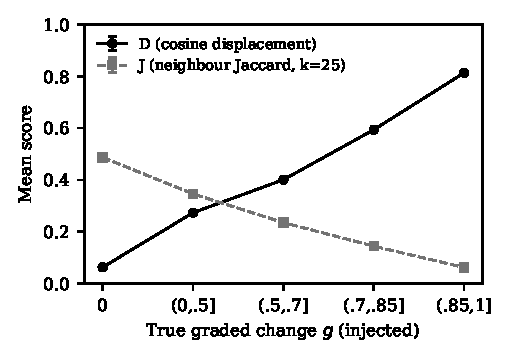
\includegraphics[width=0.84\linewidth]{fig1_dose_response.pdf}
\caption{Dose-response trajectory of $D$ and $J$ against ground-truth injected shift $g$ (Exp. 1; mean $\pm$ SD across 20 stochastic draws).}
\label{fig:dose_response}
\end{figure}

\begin{table}[t]
\caption{Shift Detection Accuracy on Synthetic Lexica (Exp. 1, AUC, Mean $\pm$ SD, $R=20$)}
\label{tab:exp1_auc}
\centering
\begin{tabular}{lc|lc}
\toprule
\textbf{Metric} & \textbf{AUC} & \textbf{Metric} & \textbf{AUC} \\
\midrule
$D$ & $0.967 \pm 0.002$ & $E_D$ & $0.985 \pm 0.002$ \\
$J$ ($k=25$) & $0.839 \pm 0.005$ & $E_J$ & $0.857 \pm 0.006$ \\
$I$ ($\alpha=0.5$) & $0.930 \pm 0.004$ & LSI (Prototype) & $0.949 \pm 0.003$ \\
$I$ ($\alpha=0.25/0.75$) & $0.885 / 0.961$ & $J$ ($k=10/50$) & $0.834 / 0.908$ \\
\bottomrule
\end{tabular}
\end{table}

\textbf{Confound Attenuation.} Word token frequency introduces an acute representational confound: among stable terms, raw displacement exhibited a strong negative correlation with log frequency ($\rho = -0.806 \pm 0.020$). Decile null calibration eliminated this bias, reducing correlation to $0.062 \pm 0.058$. As shown in Fig.~\ref{fig:decile_null}, the null floor expands exponentially in low-frequency bands, where the 95th percentile null displacement (0.583) exceeds the empirical mean displacement of authentic shifting words (0.488).

\textbf{Cautionary Findings.} (1) A naive per-word decision boundary flagging terms above the 95th percentile null floor yielded an unacceptable 43.5\% false positive rate on stable terms, demonstrating that split-half baselines serve as cohort adjustment devices rather than discrete word-level hypothesis tests. (2) Composite metric $I$ failed to surpass raw $D$, as detection performance scaled monotonically with the weight assigned to $D$. (3) Alignment computed strictly on function words ($N_A=60$, $d=50$) degraded catastrophically (AUC $0.470 \pm 0.032$), demonstrating that anchor cardinality must substantially exceed embedding dimensionality.

\begin{figure}[t]
\centering
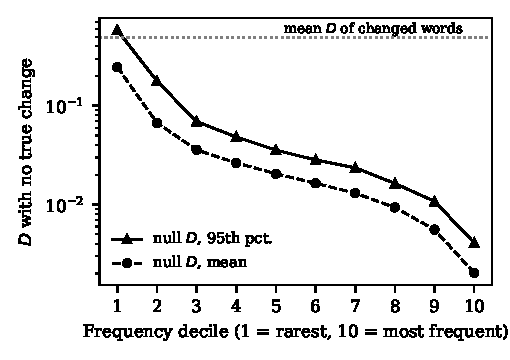
\includegraphics[width=0.84\linewidth]{fig2_null_by_decile.pdf}
\caption{Null displacement across empirical word frequency deciles among unchanged terms (Exp. 1; Decile 1 = rarest, 10 = most frequent).}
\label{fig:decile_null}
\end{figure}

\subsection{Experiment 2: Paired Domain Inference}
Across 100 simulated worlds evaluating paired general and statutory arms, condition S1 (true statutory inertia: $p_{\text{gen}}=0.30, p_{\text{stat}}=0.10$) achieved 100\% rejection power in the predicted direction (Table~\ref{tab:exp2_inference}). In condition S3, injecting 50\% copied statutory text induced a significant artificial inertia effect ($\Delta E_D = +0.064$, rejected in 100\% of worlds), which was entirely eliminated ($\Delta E_D = +0.001$, 9\% rejection) after MinHash deduplication (Fig.~\ref{fig:inference_bars}).

Under the sharp null (S2: $p_{\text{gen}} = p_{\text{stat}} = 0.20$), calibrated displacement $E_D$ maintained appropriate size, rejecting the null in 7\% of realizations (nominal 5\%). Conversely, neighbor overlap $J$ exhibited severe anti-conservative bias, rejecting the null in 43\% of worlds due to correlated neighbor-graph dependencies under bootstrap resampling.

\begin{table}[t]
\caption{Inference Across 100 Simulated Worlds (Common Anchors)}
\label{tab:exp2_inference}
\centering
\setlength{\tabcolsep}{3.5pt}
\begin{tabular}{lccccc}
\toprule
 & \textbf{Mean} & \multicolumn{4}{c}{\textbf{Fraction of Worlds with 95\% CI Excluding 0}} \\
\cmidrule{3-6}
\textbf{Condition} & $\Delta E_D$ & Raw $D$ & Calibrated $D$ & Calibrated $J$ & Domain $D$ \\
\midrule
S1 True Effect & $+0.104$ & 1.00 & 1.00 & 1.00 & 1.00 \\
S2 Null & $+0.001$ & 0.09 & 0.07 & 0.43 & 0.10 \\
S3 Copy Full & $+0.064$ & 1.00 & 1.00 & 1.00 & 1.00 \\
S3 Deduplicated & $+0.001$ & 0.11 & 0.09 & 0.44 & 0.11 \\
S4 Size Mismatch & $+0.004$ & 0.10 & 0.05 & 0.46 & 0.05 \\
\bottomrule
\end{tabular}
\end{table}

\begin{figure}[t]
\centering
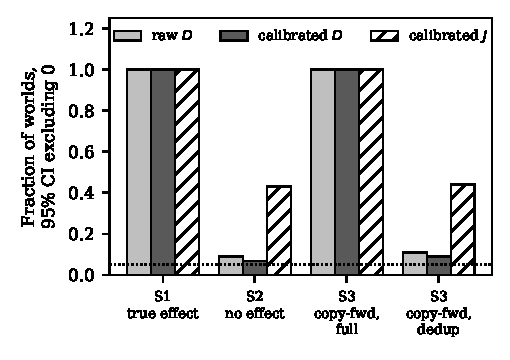
\includegraphics[width=0.84\linewidth]{fig3_inference.pdf}
\caption{Fraction of simulated worlds rejecting the null hypothesis across conditions S1--S3. Dotted line denotes nominal 5\% level.}
\label{fig:inference_bars}
\end{figure}

\subsection{Experiment 3: SemEval-2020 Real Benchmark}
\label{sec:semeval}
We evaluated the protocol on the SemEval-2020 Task 1 English graded benchmark \cite{schlechtweg2020semeval}, utilizing lemmatized CCOHA historical (1810--1860) and modern (1960--2010) slices across 37 target terms with human graded annotations. Models were trained under equal budgets ($n=3.28\times 10^6$ tokens) with PPMI-SVD ($d=100$, 2000 anchors, $k=25$).

Raw displacement $D$ and neighborhood overlap $-J$ correlate moderately with human judgments ($\rho = 0.345$ and $0.396$, Table~\ref{tab:semeval}). When frequency calibration was restricted to target terms alone, small-sample instability severely degraded performance ($E_D$ variance expanded to $\pm 0.165$). Conversely, estimating the empirical null distribution over the shared background candidate pool ($N=3000$, \texttt{--null-mode pool}) stabilized calibration, yielding consistent alignment ($\rho = 0.348 \pm 0.048$ for $E_D$; $\rho = 0.340 \pm 0.028$ for $E_J$). This confirms that noise floor calibration on authentic corpora requires an adequate background vocabulary pool to avoid sparse-decile sampling distortions.

\begin{table}[t]
\caption{SemEval-2020 English: Spearman Rank Correlation With Human Gold Scores ($n=37$, Two-Sided $p$-Value in Parentheses)}
\label{tab:semeval}
\centering
\setlength{\tabcolsep}{3.0pt}
\small
\resizebox{\columnwidth}{!}{%
\begin{tabular}{lcccc}
\toprule
\textbf{Metric} & \textbf{Run 1} & \textbf{Run 2} & \textbf{Run 3} & $\mathbf{Mean \pm SD}$ \\
\midrule
$D$ (Raw) & 0.408 (.012) & 0.304 (.067) & 0.324 (.050) & $0.345 \pm 0.055$ \\
$E_D$ (Target Deciles) & 0.461 (.004) & 0.287 (.085) & 0.131 (.440) & $0.293 \pm 0.165$ \\
$E_D$ (Candidate Pool) & 0.401 (.014) & 0.309 (.063) & 0.335 (.043) & $0.348 \pm 0.048$ \\
$-J$ (Raw) & 0.372 (.023) & 0.449 (.005) & 0.366 (.026) & $0.396 \pm 0.046$ \\
$E_J$ (Candidate Pool) & 0.317 (.056) & 0.371 (.024) & 0.332 (.044) & $0.340 \pm 0.028$ \\
\bottomrule
\end{tabular}%
}
\end{table}


\section{Discussion and Operational Guidelines}
The experimental findings establish specific operational criteria for future diachronic legal language studies:
\begin{itemize}
    \item \textbf{Metric Priority:} Continuous cosine displacement $D$ under robust anchor sets ($N_A \gg d$) exhibits superior stability and inference validity compared to discrete neighborhood overlap $J$.
    \item \textbf{Inheritance Controls:} Legislative deduplication is mandatory; failure to filter copied statutory text introduces substantial false-positive inertia effects.
    \item \textbf{Calibration Pools:} Frequency-decile noise adjustment must draw from broad background candidate distributions rather than isolated evaluation subsets.
\end{itemize}

\section{Limitations}
Synthetic language models assume localized topical migration, omitting complex polysemy, syntactic shifts, and historical OCR artifacts. Furthermore, while the SemEval benchmark provides empirical validation on natural text, its targets reflect general historical vocabulary. Validating true statutory semantic inertia requires running this pipeline on authentic legislative session laws paired with expert legal-historical annotations.

\section{Reproducibility and Ethics}
{\sloppy The complete experimental harness (\texttt{sim.py}, \texttt{run\_exp1.py}, \texttt{run\_exp2.py}, \texttt{real\_pipeline.py}, \texttt{make\_figures.py}) and benchmark evaluation logs are available under open-source licensing at \path{https://github.com/Haidriyam/statutory-semantic-intertia} and archived on Zenodo (DOI: 10.5281/zenodo.23613023). All stochastic seeds are fixed. Computational execution requires approximately 25 minutes on a standard CPU core.\par}

\textbf{Ethical Disclosure:} In accordance with AI transparency guidelines, Claude (Anthropic) was utilized strictly for syntactical polishing, bibliographic formatting, and script modularization. The human authors conceived the study, derived the formal mathematical models, developed and verified all experimental scripts, and conducted the forensic repository audit.

\section{Conclusion}
Earlier prototype implementations demonstrated alignment mathematics over hand-crafted sentences, but did not measure legal language. We provide a rigorous, calibrated measurement protocol that separates embedding stability from textual copy-forward artifacts and doctrinal legal meaning. Controlled experiments establish that the protocol isolates genuine semantic drift, eliminates frequency distortions, and neutralizes statutory duplication. The protocol establishes the necessary empirical machinery to test whether legislative language demonstrates authentic semantic inertia.

\bibliographystyle{IEEEtran}
\begin{thebibliography}{00}

\bibitem{hamilton2016diachronic}
W.~L. Hamilton, J.~Leskovec, and D.~Jurafsky, ``Diachronic word embeddings reveal statistical laws of semantic change,'' in \emph{Proc. 54th Annu. Meeting Assoc. Comput. Linguistics (ACL)}, 2016, pp. 1489--1501.

\bibitem{scalia2012reading}
A.~Scalia and B.~A. Garner, \emph{Reading Law: The Interpretation of Legal Texts}.\hskip 1em plus 0.5em minus 0.4em\relax St. Paul, MN, USA: West, 2012.

\bibitem{eskridge1987dynamic}
W.~N. Eskridge, Jr., ``Dynamic statutory interpretation,'' \emph{Univ. Pennsylvania Law Rev.}, vol. 135, no.~6, pp. 1479--1555, 1987.

\bibitem{hart1961concept}
H.~L.~A. Hart, \emph{The Concept of Law}.\hskip 1em plus 0.5em minus 0.4em\relax Oxford, U.K.: Clarendon Press, 1961.

\bibitem{antoniak2018evaluating}
M.~Antoniak and D.~Mimno, ``Evaluating the stability of embedding-based word similarities,'' \emph{Trans. Assoc. Comput. Linguistics}, vol.~6, pp. 107--119, 2018.

\bibitem{wendlandt2018factors}
L.~Wendlandt, J.~K. Kummerfeld, and R.~Mihalcea, ``Factors influencing the surprising instability of word embeddings,'' in \emph{Proc. NAACL-HLT}, 2018, pp. 2092--2102.

\bibitem{hellrich2016bad}
J.~Hellrich and U.~Hahn, ``Bad company---neighborhoods in neural embedding spaces considered harmful,'' in \emph{Proc. COLING}, 2016, pp. 2785--2796.

\bibitem{dubossarsky2017outta}
H.~Dubossarsky, D.~Weinshall, and E.~Grossman, ``Outta control: Laws of semantic change and inherent biases in word representation models,'' in \emph{Proc. EMNLP}, 2017, pp. 1136--1145.

\bibitem{gonen2020simple}
H.~Gonen, G.~Jawahar, D.~Seddah, and Y.~Goldberg, ``Simple, interpretable and stable method for detecting words with usage change across corpora,'' in \emph{Proc. 58th Annu. Meeting ACL}, 2020, pp. 538--555.

\bibitem{hamilton2016cultural}
W.~L. Hamilton, J.~Leskovec, and D.~Jurafsky, ``Cultural shift or linguistic drift? Comparing two computational measures of semantic change,'' in \emph{Proc. Conf. Empirical Methods Natural Language Process. (EMNLP)}, 2016, pp. 2116--2121.

\bibitem{mikolov2013efficient}
T.~Mikolov, K.~Chen, G.~Corrado, and J.~Dean, ``Efficient estimation of word representations in vector space,'' \emph{arXiv preprint arXiv:1301.3781}, 2013.

\bibitem{schonemann1966generalized}
P.~H. Sch{\"o}nemann, ``A generalized solution of the orthogonal Procrustes problem,'' \emph{Psychometrika}, vol.~31, no.~1, pp. 1--10, 1966.

\bibitem{kutuzov2018diachronic}
A.~Kutuzov, L.~{\O}vrelid, T.~Szymanski, and E.~Velldal, ``Diachronic word embeddings and semantic shifts: A survey,'' in \emph{Proc. COLING}, 2018, pp. 1384--1397.

\bibitem{tahmasebi2021survey}
N.~Tahmasebi, L.~Borin, and A.~Jatowt, ``Survey of computational approaches to lexical semantic change detection,'' in \emph{Computational Approaches to Semantic Change}.\hskip 1em plus 0.5em minus 0.4em\relax Berlin, Germany: Language Science Press, 2021, pp. 1--91.

\bibitem{kulkarni2015statistically}
V.~Kulkarni, R.~Al-Rfou, B.~Perozzi, and S.~Skiena, ``Statistically significant detection of linguistic change,'' in \emph{Proc. 24th Int. Conf. World Wide Web (WWW)}, 2015, pp. 625--635.

\bibitem{shoemark2019room}
P.~Shoemark, F.~Ferdousi~Liza, D.~Nguyen, S.~Hale, and B.~McGillivray, ``Room to Glo: A systematic comparison of semantic change detection approaches with word embeddings,'' in \emph{Proc. EMNLP-IJCNLP}, 2019, pp. 66--76.

\bibitem{schlechtweg2020semeval}
D.~Schlechtweg, B.~McGillivray, S.~Hengchen, H.~Dubossarsky, and N.~Tahmasebi, ``SemEval-2020 Task 1: Unsupervised lexical semantic change detection,'' in \emph{Proc. 14th Int. Workshop Semantic Evaluation}, 2020, pp. 1--23.

\bibitem{dubossarsky2019time}
H.~Dubossarsky, S.~Hengchen, N.~Tahmasebi, and D.~Schlechtweg, ``Time-out: Temporal referencing for robust modeling of lexical semantic change,'' in \emph{Proc. 57th Annu. Meeting ACL}, 2019, pp. 457--470.

\bibitem{levy2014neural}
O.~Levy and Y.~Goldberg, ``Neural word embedding as implicit matrix factorization,'' in \emph{Adv. Neural Inf. Process. Syst. (NIPS)}, 2014, pp. 2177--2185.

\bibitem{soni2021follow}
S.~Soni, K.~Lerman, and J.~Eisenstein, ``Follow the leader: Documents on the leading edge of semantic change get more citations,'' \emph{J. Assoc. Inf. Sci. Technol.}, vol.~72, no.~4, pp. 478--492, 2021.

\bibitem{braun2022tracking}
D.~Braun, ``Tracking semantic shifts in German court decisions with diachronic word embeddings,'' in \emph{Proc. Natural Legal Language Process. Workshop (NLLP)}, 2022, pp. 218--227.

\bibitem{wang2026aetas}
Q.~Wang, ``AETAS: Analysis of Evolving Temporal Affect and Semantics for Legal History,'' \emph{arXiv preprint arXiv:2512.22196}, 2026.

\bibitem{lee2018judging}
T.~R. Lee and S.~C. Mouritsen, ``Judging ordinary meaning,'' \emph{Yale Law J.}, vol. 127, no.~4, pp. 788--879, 2018.

\bibitem{davies2012expanding}
M.~Davies, ``Expanding horizons in historical linguistics with the 400-million word Corpus of Historical American English,'' \emph{Corpora}, vol.~7, no.~2, pp. 121--157, 2012.

\bibitem{broder1997resemblance}
A.~Z. Broder, ``On the resemblance and containment of documents,'' in \emph{Proc. Compression and Complexity of Sequences}, 1997, pp. 21--29.

\end{thebibliography}

\end{document}